\documentclass[a4paper,10pt]{article}
%\documentclass[a4paper,10pt]{scrartcl}

\usepackage[utf8]{inputenc}
\usepackage{graphicx}
\usepackage{geometry}
\usepackage[table]{xcolor}  

 \geometry{
 a4paper,
 left=20mm,
 right=20mm,
 top=20mm,
 bottom=15mm,
 }
\pagestyle{empty}

\title{CIPSI Algorithm}
\author{}
\date{\today}

\begin{document}
\maketitle

In the CIPSI algorithm, the determinant space (generated by ijkl/fock) is partitioned into 3 subspaces.
The subspace S is the reference space chosen by the user. The obtained submatrix is then diagonalized to get netat energies corresponding to the lowest states. The contribution of the determinants outside of space S is evaluated with a second order perturbative algorithm.
The subspace M is formed by the determinants with a contribution superior to a given threshold. The matrix formed by the association S+M contained all determinants deemed important and is the one which will be diagonalized at the end of the procedure.
The subspace P is formed by the leftovers determinants, they will be taken into account by including their second order perturbative contribution to the energy.


In the current implementation, the \textit{cip} binary generate the subspace S and compute the perturbation of other determinants, the \textit{moy} binary construct the matrix of S+M and the \textit{bd} binary diagonalize said matrix and add various corrections (perturbation, Davidson correction, …) to the final energies.

\section{Relevant options to run a perturbative CI or a Full-CI :}

Namelists found in input file *sym.dat

\underline{\textbf{Namelist “icinp”:}}
\begin{itemize}
 \item LECDET : how to construct the reference space. 2 : the space is read from listing of a previous computation. 4 : generate a CAS with user given information on symmetry / active orbitals.
 \item NOAC : only with lecdet=4. number of active orbital to generate the CAS.
 \item NUMAC : only with lecdet=4. List of index of each active orbital (information on the orbitals are in the ijkl listing generated by fock). If missing the default will be to take the orbitals from 1 to noac.
 \item ITYPER : method used to compute second order perturbation. 1 : method MPB (Möller Plesset Barycentrique). 2 : method ENVP (Epstein-Nesbet Valeur Propre). Negative values : no perturbation computed (used for Full CI)
 \item ISELEC : how to select strong/weak determinant. 1 : look at the contribution on the  wavefunction. 3 : look at the contribution on the energy
 \item TEST and TAU : thresholds (in energy or amplitude depending on iselec) used to determine if the determinant is included in the listing or not.
\end{itemize}

\underline{\textbf{Namelist “moyen”:}}
\begin{itemize}
 \item TAU : threshold (in energy or amplitude depending on iselec) used to determine if the determinant is included in the M subspace.
\end{itemize}


\underline{\textbf{Namelist “option”:}}
\begin{itemize}
 \item QICTOT : true for Full CI computation, false if you use a perturbative approach. If false, second order perturbative contribution as well as additional correction (davidson) are added to the final energy.
\end{itemize}

\section{Implementation of the algorithm in Autocip\_v9}

Additional options contained in auto.in :
\begin{itemize}
 \item NOAC : value inserted in the icinp namelist. If negative a FCI calculation will be performed.
 \item ENVP\_max / NUM\_REF / TAU\_init / TAU\_step : values used to construct the subspace M. 
\end{itemize}

The program will first generate two sym.dat file containing the namelists required by the binaries : the first file is used for the first call to \textit{cip}, after that the second file (*\_loop) will be used. The first file has LECDET=4, and the given number for NOAC, the second one LECDET=2 and NOAC is not included. We also set for both ITYPER=2 (ENVP method used), a dummy value for TEST and TAU (the algorithm will modify those values with a sed command) and QICTOT=F. If the Full CI method is requested (NOAC negative or too big) then only the first .dat file is useful and set up with LECDET=4, ITYPER=-1, QICTOT=T and NOAC is given the value from the pshf output.

The algorithm is as follows :
\begin{itemize}
 \item Do the first call to \textit{cip} to generate the initial reference subspace S. TAU and TEST are set to a high value (default : 0.9) to include only a small number of determinant in the listing.
 \item Loop on \textit{cip} to increase the size of S. After a calculation the listings contain S + strong determinants. \textit{cip} read all those determinants to generate and work on a new bigger reference space S'. At each step of the loop TAU is decreased (default : multiply by 0.75 and sed the new value in the input file) so the number of determinant considered will increase. At the end of each step the size of the reference space is read in the 'f04' listing, the loop is exited once this size is big enough. The final size must be greater than netat, currently the exit condition is size $>$ num\_ref. Note that to compute the second order perturbative energies of the determinants \textit{cip} need to diagonalize the subspace S, the maximal size must therefore remain small (up to a few hundreds with current computers).
 TODO : check precision depending on the ref space size.
 \item Final call to \textit{cip} with TAU and TEST set to zero so that \textit{moy}/\textit{bd} will have informations (notably the perturbative energy ENVP) for every determinants. We also extract from the output file cip the energies ENVP(i) corresponding to the sums of second order energies contribution for all the determinants not in S. These perturbative corrections ENVP are given for each of the netat states. 
 \item Loop on \textit{moy} to select the subspace M. \textit{moy} read the reference space S as well as the perturbation of every other determinants in the various listings. TAU is initially set to the value TAU\_init. At each step, after the call to \textit{moy}, we extract from the output file moy the perturbative energy contribution ENVP\_M of the determinants included in M. (ENVP - ENVP\_M) is the contribution ENVP\_P of the ``rest'' subspace P (note : it would be more efficient to compute directly ENVP\_P, however this would require a complete overhaul of some subroutines in \textit{moy}). We look at the state with the biggest correction ENVP\_P, if this value is lower than ENVP\_max the loop is exited. Otherwise we decrease the value of TAU (multiplication by TAU\_step) and proceed with the next iteration. As we decrease TAU, the size of M will increase and the one of P will decrease, the perturbation ENVP\_P will thus also decrease.    
 \item Call to \textit{bd}. The matrix diagonalized by the davidson algorithm contain all the determinants of the subspaces S and M. 
\end{itemize}



Some remarks : 
\begin{enumerate}
 \item If NOAC is negative (Full CI mode), the program make only a single call $cip>moy>bd$ similar to Autocip\_v8.
 \item Informations on orbitals (for NUMAC) can be found in the ijkl output. By default the program add all the occupied HF-orbitals to NUMAC. It will then add the requested number of virtual orbital. For each virtual orbital the multiplication table of the point group is checked to see if a monoexcited determinant will be of the desired symmetry, otherwise the orbital is discarded. The automatic numac option is written at the beginning of the namelist and won't be used if the user supply a custom numac.
 \item While weakly coupled to the ground state, parazite state can still appear for certain geometry. Check multiplication table in ijkl to get rid of them ?
 \item The loop on \textit{cip} is fast as long as the size of S remain small. The loop on \textit{moy} also take only a few seconds. Though to gain time one can adjust the value of TAU\_init and TAU\_step. If TAU\_init is small enough the desired space M will be constructed at the first iteration. Previous calculation on the same system can be check to get a good guess on TAU.
 \item The algorithm could also be used by running $cip>moy>bd$ at each step. Instead of diagonalizing the space S, \textit{cip} read eigenvalues/eigenvectors from the previous iteration of bd. This allow bigger S space as bd use the efficient davidson algorithm while cip use a brute force lapack diagonalization. The option is however bug. In this mode \textit{cip} read some informations given by the previous \textit{cip} call as well as data from \textit{bd}. One concern the space S, the other the space S+M. As their size is incompatible the program crash.  
\end{enumerate}

\section{Modification in the CIPSI source}

\begin{description}
\item Small bugfixes in \textit{cip}/\textit{moy}/\textit{bd}/\textit{ciro}
\item fixed unitialized value of ii in ciro
\item Given routine replace by a Lapack call in \textit{cip} and \textit{ciro}.
\item allocation of perturbation matrix (hef, hefen ...) in moy/morue.f changed from ndetz*(ndetz+1)/2 to nhefz
\item If the number of determinant is smaller than ncper, \textit{bd} will use a direct lapack diagonalization instead of the Davidson algorithm.
\item Added in \textit{bd} output the norm of the eigenvectors for checks : partial value with the ncper first component as well as total value (supposed to be 1).
\item Added a final ouput in extr.f of \textit{bd} so that the output has the same structure for qictot=F and T
\item If the eigenvalues of the effective/exact Hamiltonian don't match in extr.f, the computation of Davidson correction/renormalisation are skipped.  
\item Added the binary \textit{spin} that read \textit{bd} listings and compute for each states the value of $\Psi | S^2 | \Psi$. The value of 2S+1 for each state is given in the output. This routine is mostly a copy/paste of various subroutines found in \textit{cip}. Note that this binary is quite slow to execute, sometimes slower than bd, as recontructing the whole $S^2$ matrix takes times. 
\item Added the listing 64 '\_det\_spin' to \textit{moy}. This file is needed by the binary \textit{spin} and contain information on each determinants. (Previously we had listings for the reference space from \textit{cip} but some informations on the determinants of space M were computed by \textit{moy} but not saved on files)
\item Added an error tag in ijkl output when the routine rotat2.f stop. The tag can be used to increase/decrease trec and restart ijkl automatically. 
\item Added mrec to ``vpol'' namelist (cval) (needed for a memory allocation). The needed value can be read in pshf output. 
\item new : all blocks in unit=8 (ijkl,cval and scf) are read and stored in memory at the beginning of the computation
\item ERROR ? not fixed in pshf : dname, fname on atom.f  are uninitialized. set to blanc as temporary fix
\item pshf/cale.f : "alpha" replaced by "amix"
\item pshf/dafile.f : ante initialized to "  pshf"
\item pshf/atom.f loop on dname changed (from i=1,7 to i=1,6), dfg2 initialazed to blanc
\item pshf/ dafile.f;daclose.f;ptgrp.f;cale.f : corrected some declarations ; logical ymono ; character*8 aname,direct,title
\item increase dimension of iodb to 5000 (allow for more iteration)
\item pshf/scf.f;qmat.f : replaced hdiag subroutine by a lapack call (diagonaliser.f90)
\end{description}

\section{Benchmark test}

\subsection{KCS}

Computation made to obtain 20 $\Sigma$ states of KCs between $R=4.2~a.u.$ and $R=30~a.u.$. In the input files noac was set to 1, Tau\_init to 0.5 and tau\_step to 0.75. ENVP\_MAX was resp. $10^{-4}~a.u.$, $10^{-5}~a.u.$, $10^{-6}~a.u.$ or Full-CI was used. Computation time were resp. $27115.8~s$, $27975.9~s$ and $24173.6~s$ (the $10^{-4}$ test crashed during the sorting, so no total time values)

 \begin{figure*}[htbp]
  \begin{center}
        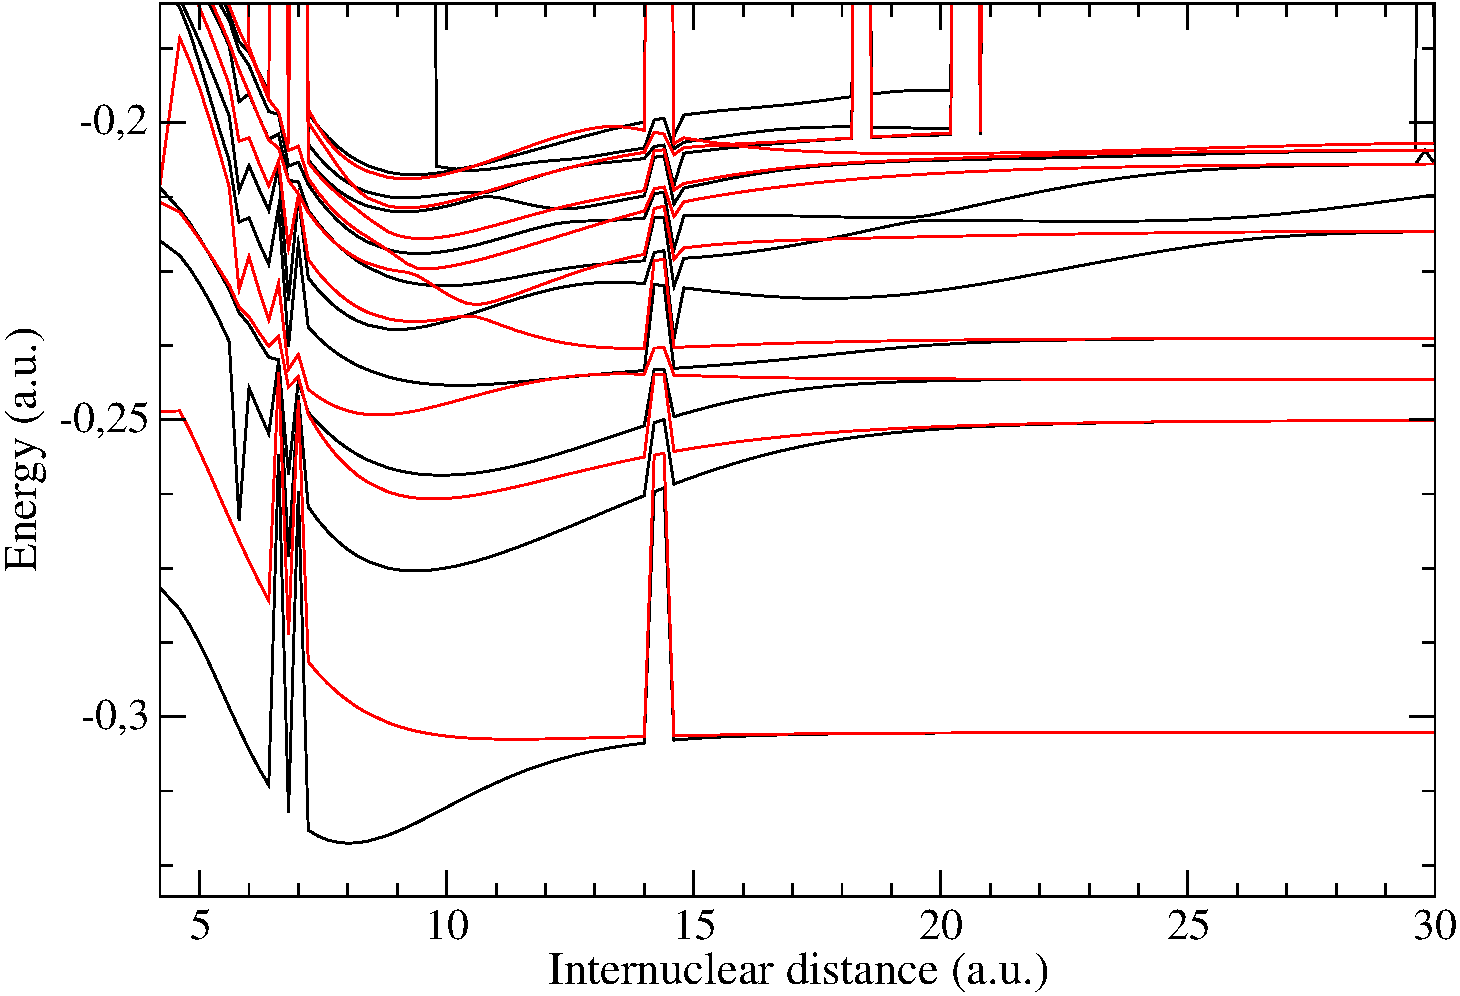
\includegraphics[width=0.7\textwidth]{fig/KCs_tau5.pdf}
    \caption{\label{PEC} \small PEC computed for $ENVP=10^{-5}~a.u.$.}
  \end{center}
\end{figure*}

\pagebreak

 \begin{figure*}[ht!]
  \begin{center}
        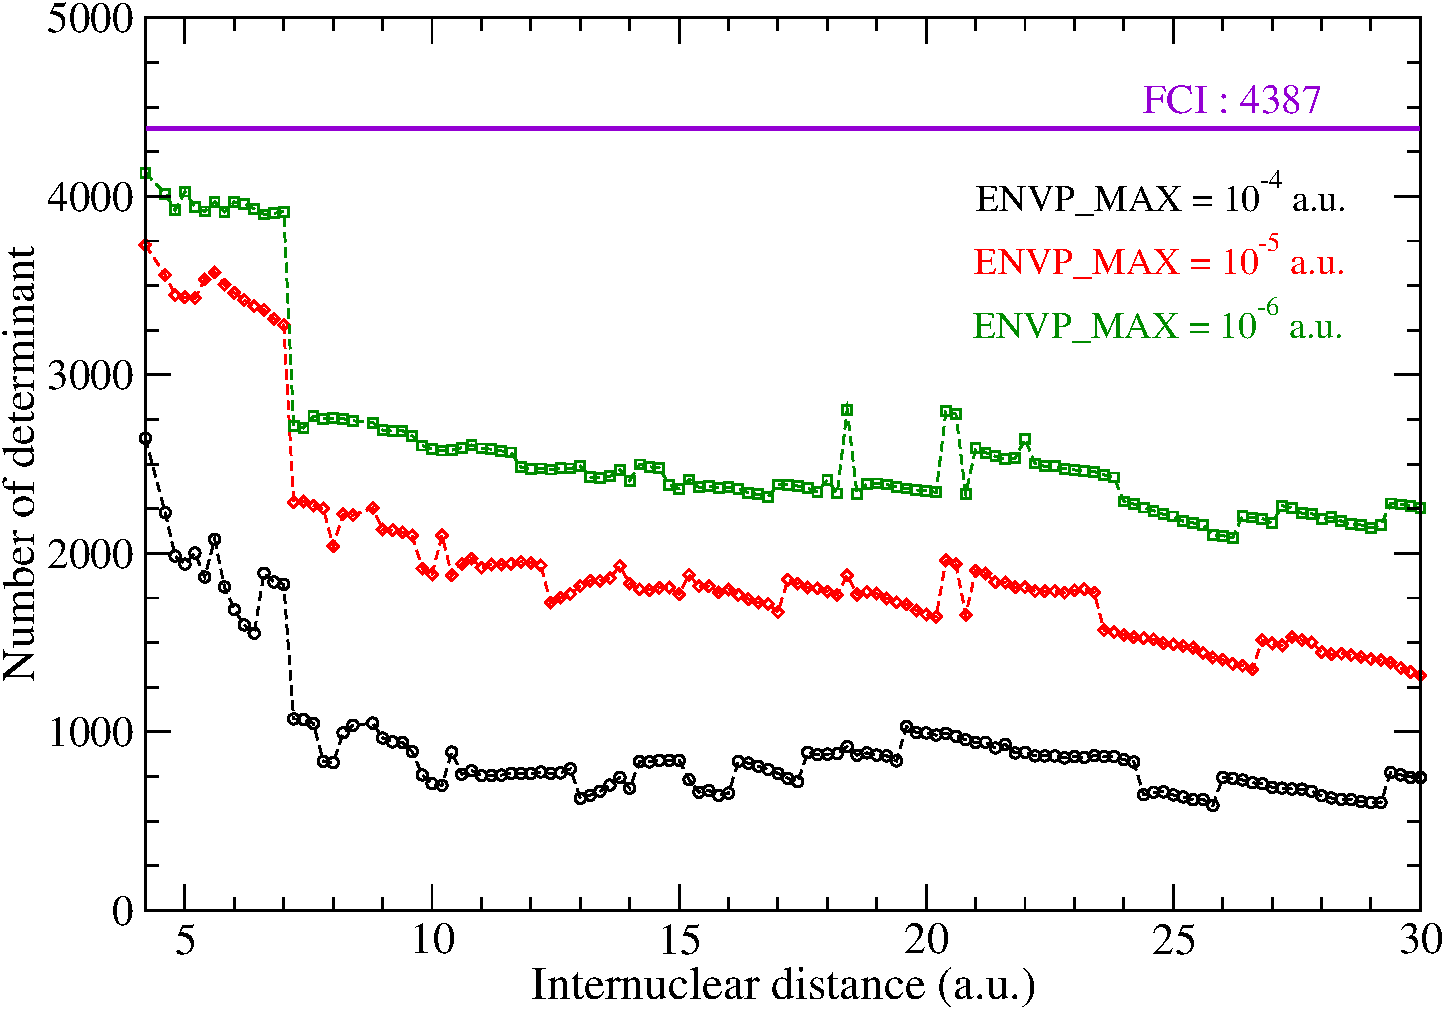
\includegraphics[width=0.8\textwidth]{fig/ndet.pdf}
    \caption{\label{ndet} \small Number of determinant for each set of input parameters.}
  \end{center}
\end{figure*}

 \begin{figure*}[hb!]
  \begin{center}
        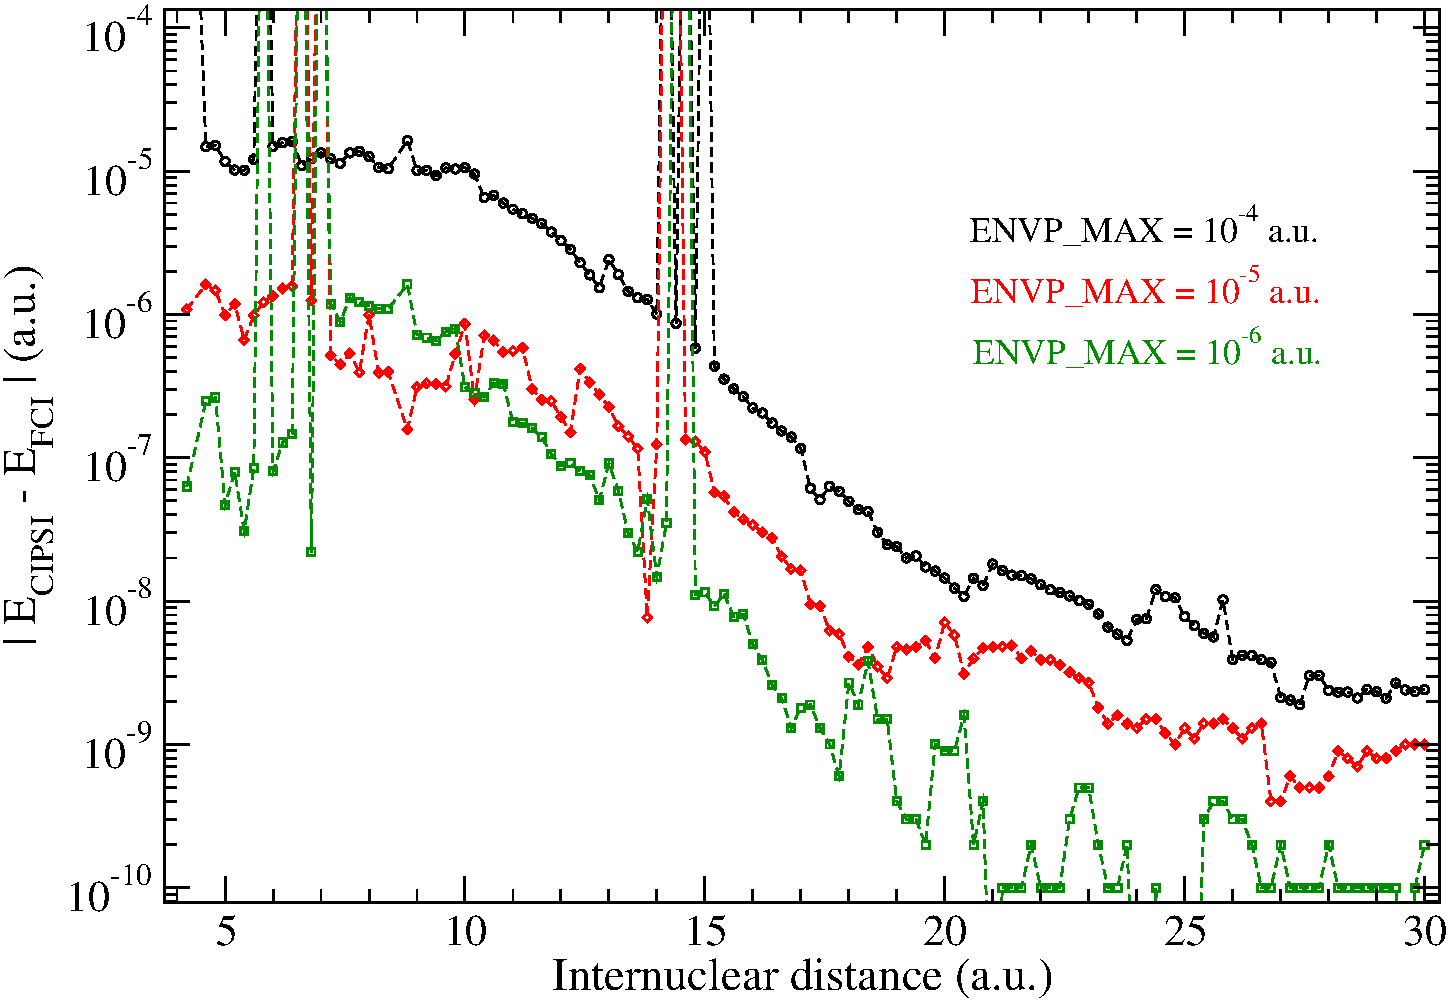
\includegraphics[width=0.8\textwidth]{fig/ssp1_convergence.pdf}
    \caption{\label{convergence} \small Comparaison between CIPSI ground state energy and the FCI one for each set of parameter.}
  \end{center}
\end{figure*}

\pagebreak


 \begin{figure*}[ht!]
  \begin{center}
        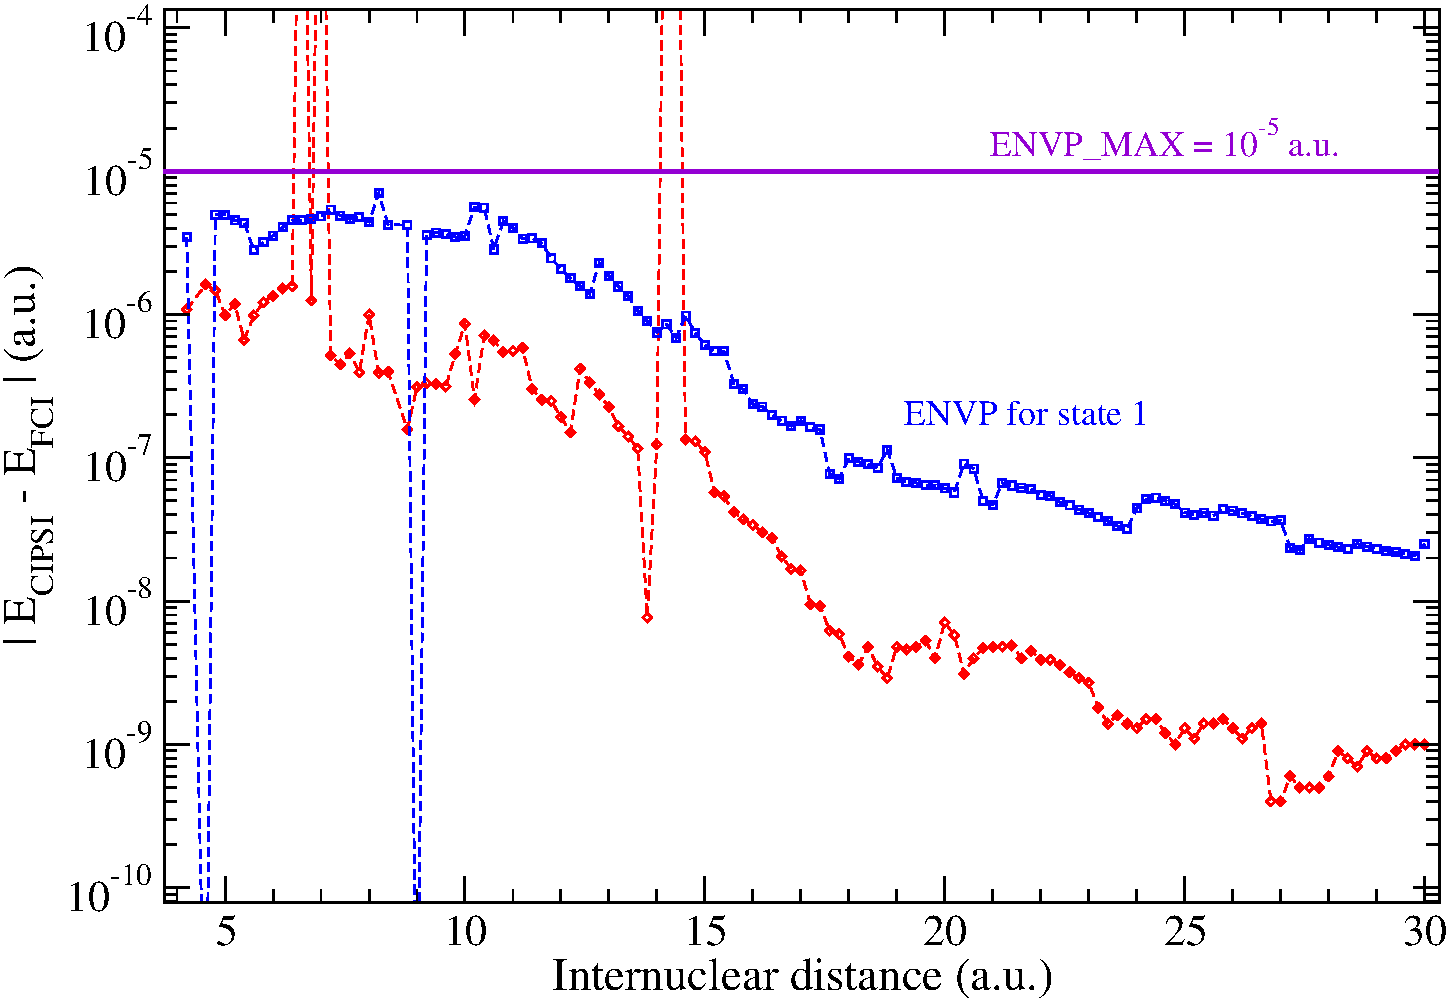
\includegraphics[width=0.8\textwidth]{fig/ssp1_tau5.pdf}
    \caption{\label{ssp1} \small Contribution of the subspace P to the ground state energy. ($ENVP=10^{-5}~a.u.$)}
  \end{center}
\end{figure*}

 \begin{figure*}[hb!]
  \begin{center}
        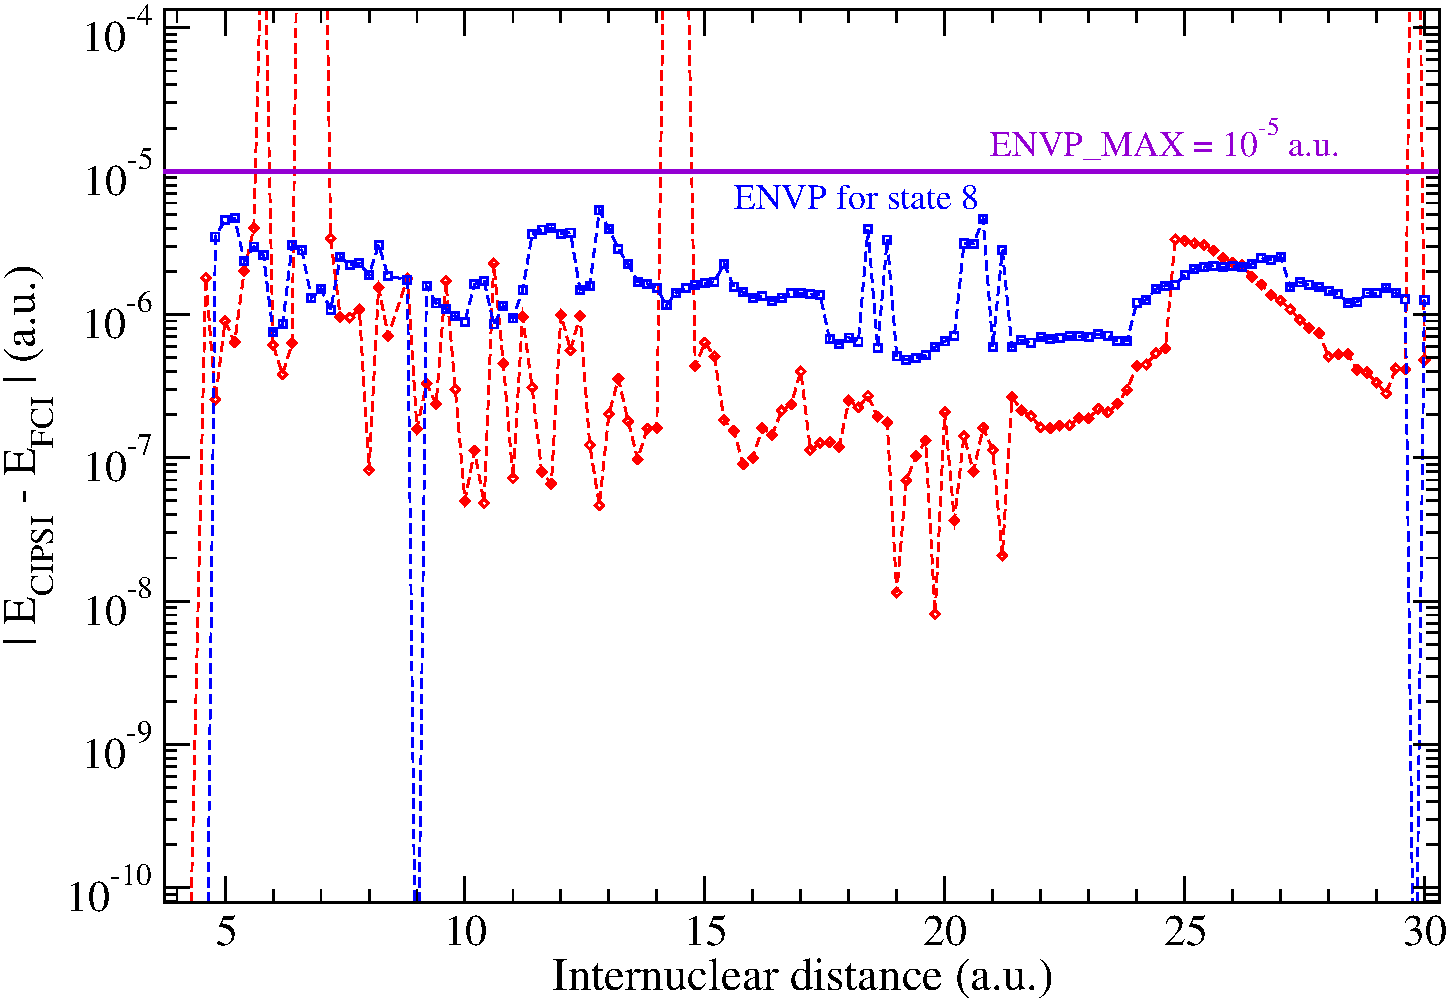
\includegraphics[width=0.8\textwidth]{fig/ssp8_tau5.pdf}
    \caption{\label{ssp8} \small same as fig.\ref{ssp1} but for the (8)$\Sigma^+$ state. ($ENVP=10^{-5}~a.u.$)}
  \end{center}
\end{figure*}

\pagebreak

 \begin{figure*}[ht!]
  \begin{center}
        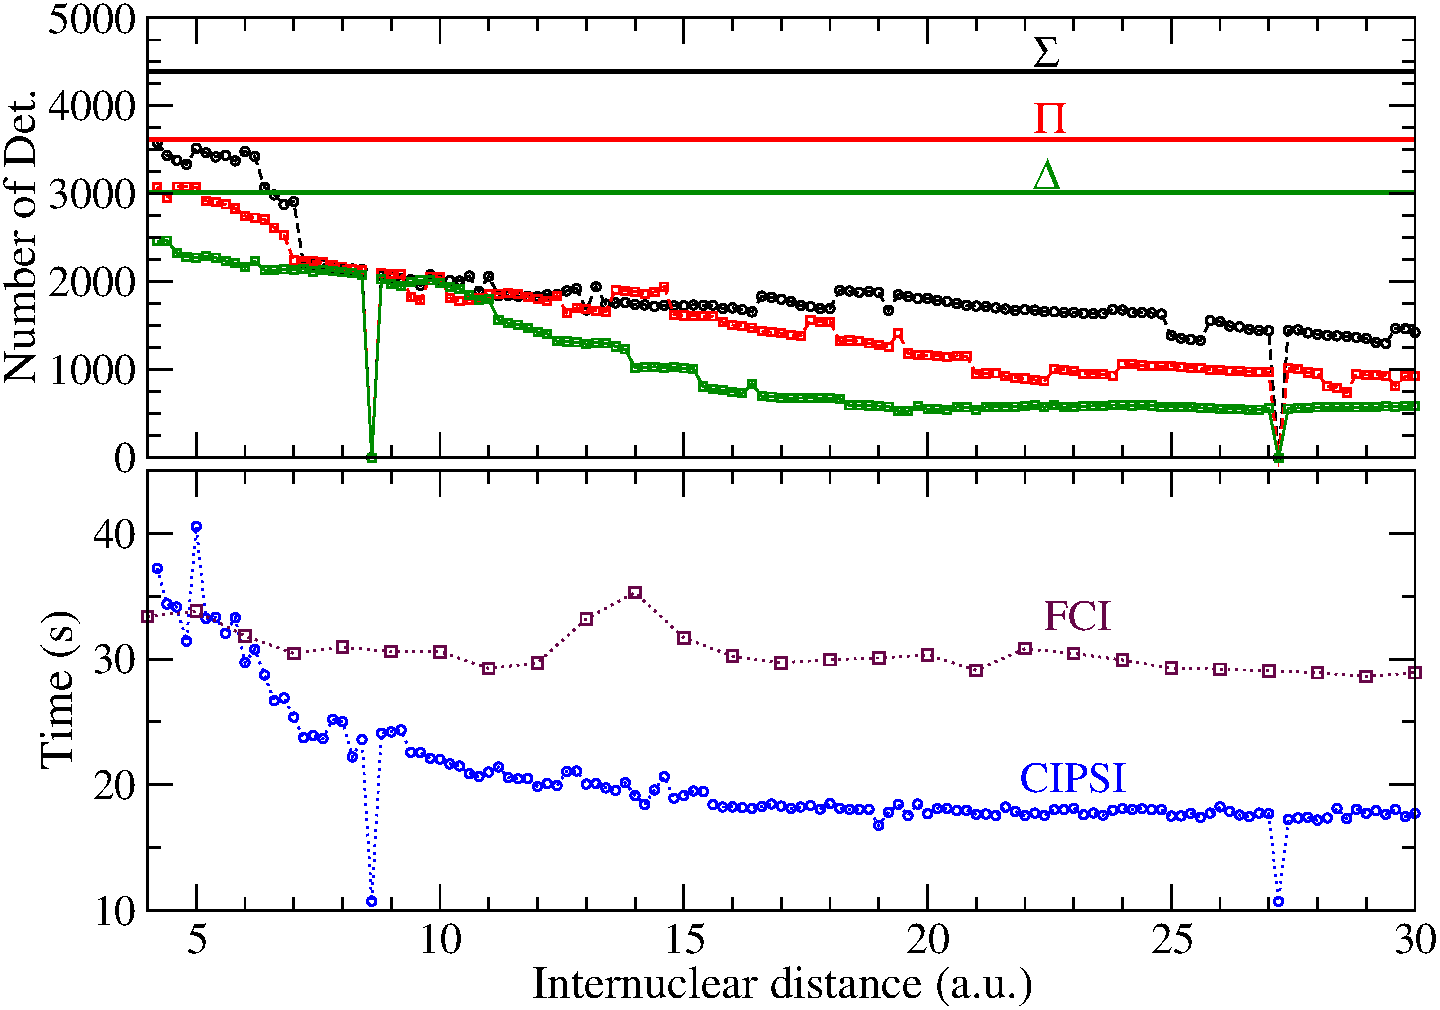
\includegraphics[width=0.8\textwidth]{fig/time_laptop.pdf}
    \caption{\label{time_p} \small Full calculation on my laptop for 20 $\Sigma$/$\Pi$/$\Delta$. Number of determinants and computation time for each geometry (including the full chain pshf to ciro)($ENVP=10^{-5}~a.u.$)}
  \end{center}
\end{figure*}

 \begin{figure*}[hb!]
  \begin{center}
        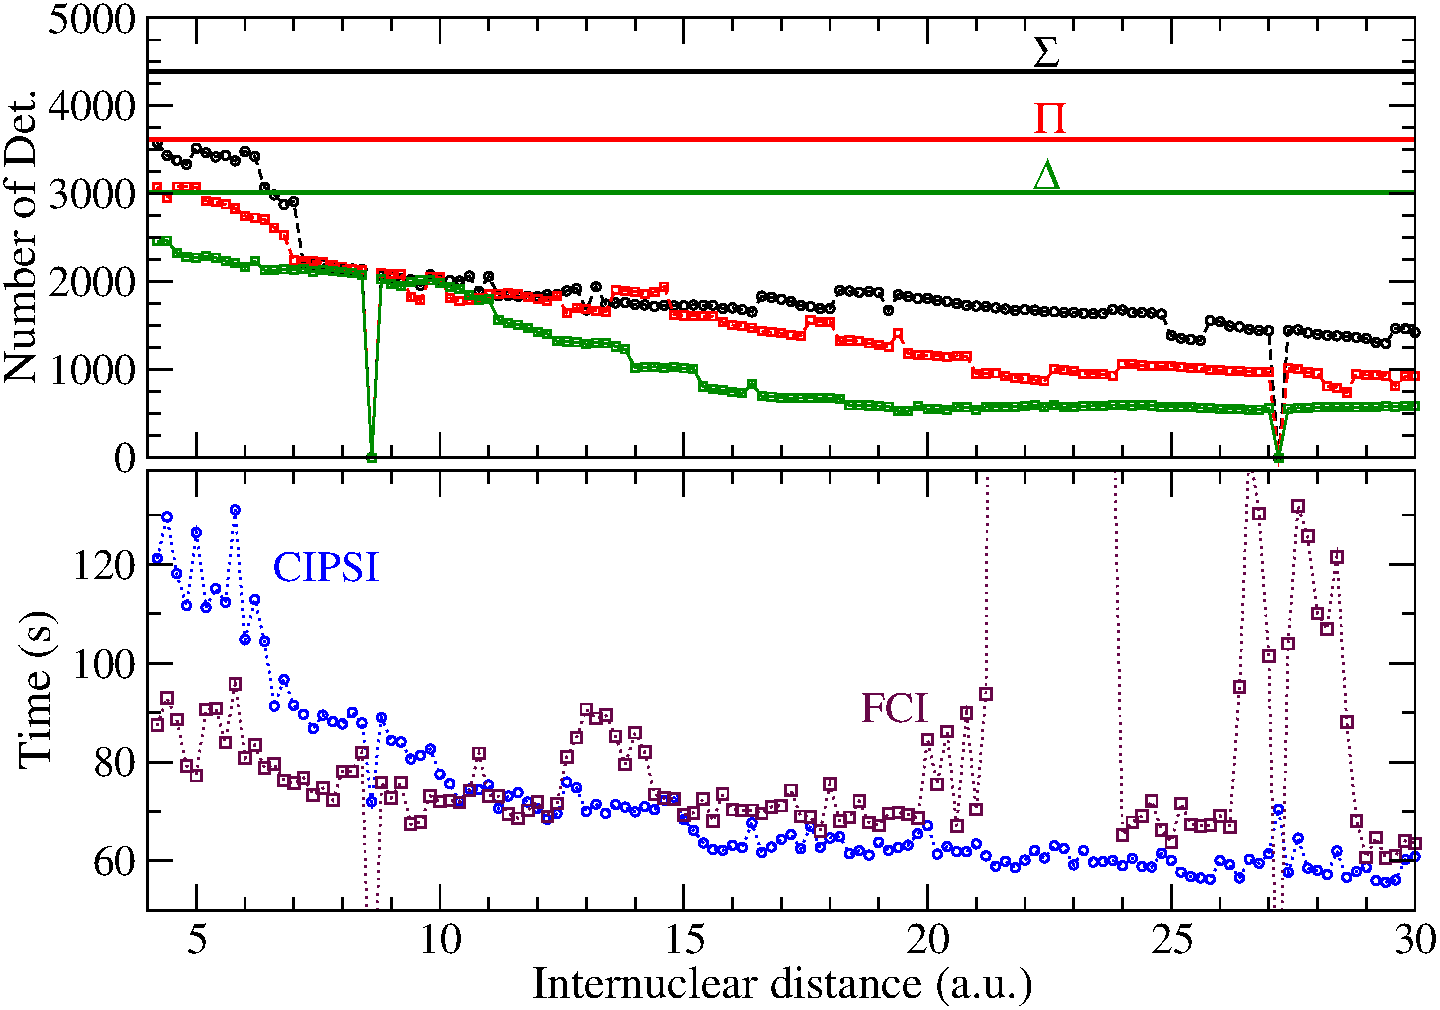
\includegraphics[width=0.8\textwidth]{fig/time_GMPCS.pdf}
    \caption{\label{time_l} \small Full calculation on GMPCS for 20 $\Sigma$/$\Pi$/$\Delta$. Number of determinants and computation time for each geometry (including the full chain pshf to ciro)($ENVP=10^{-5}~a.u.$)}
  \end{center}
\end{figure*}

\pagebreak

 \begin{figure*}[ht!]
  \begin{center}
        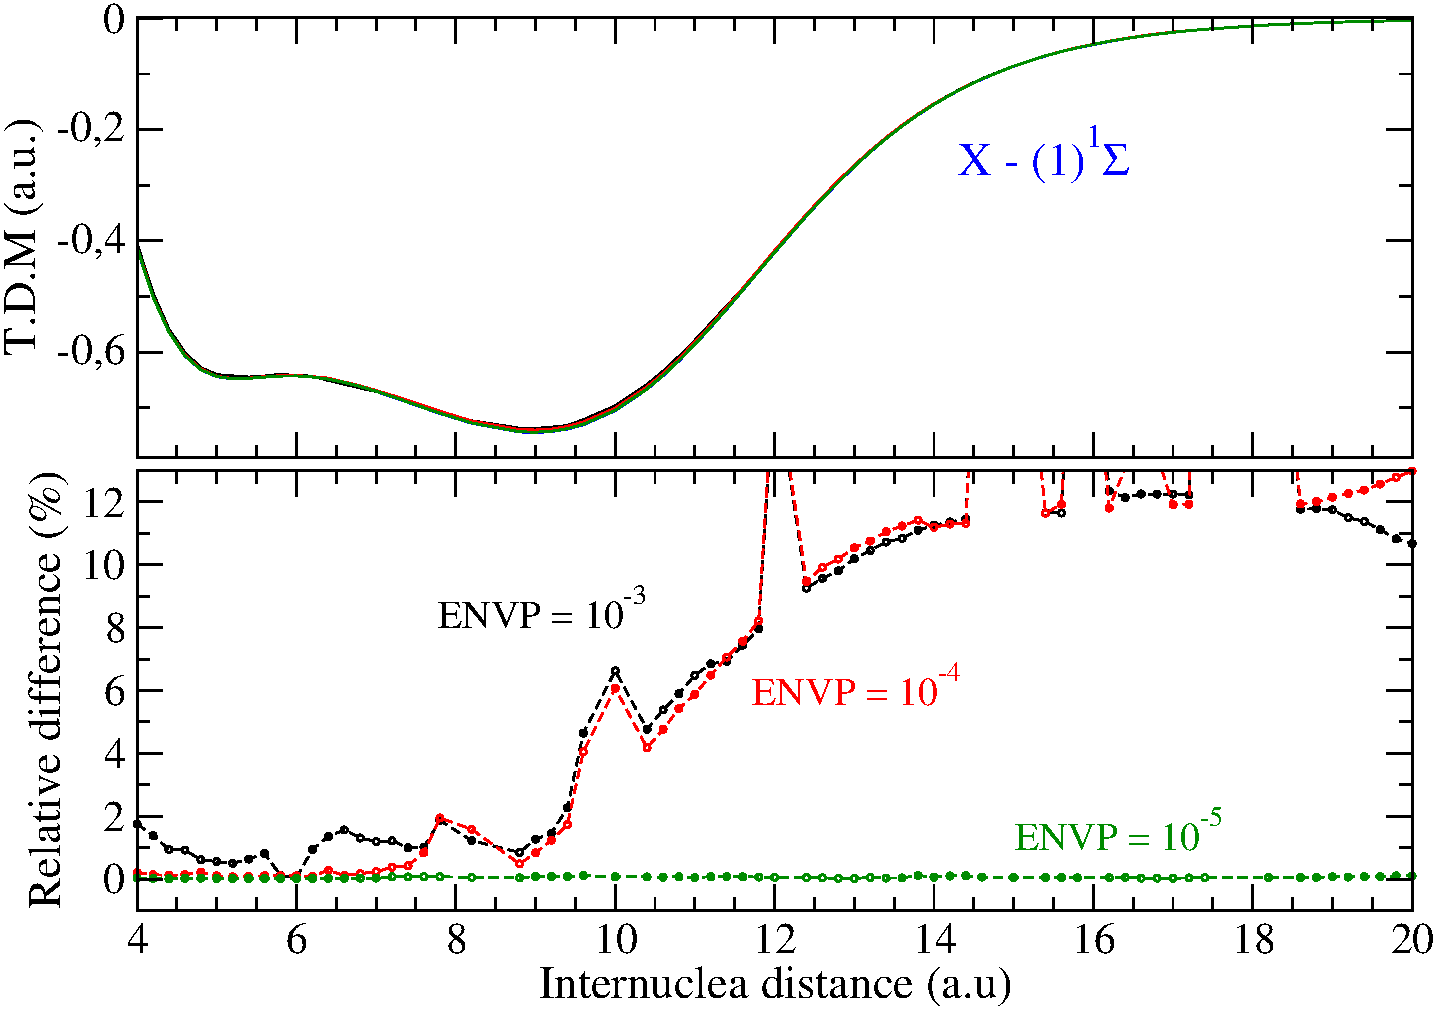
\includegraphics[width=0.8\textwidth]{fig/tdm_1ssp.pdf}
    \caption{\label{tdm1} \small Comparaison of permanent dipole moment computed with different value of ENVP}
  \end{center}
\end{figure*}

 \begin{figure*}[hb!]
  \begin{center}
        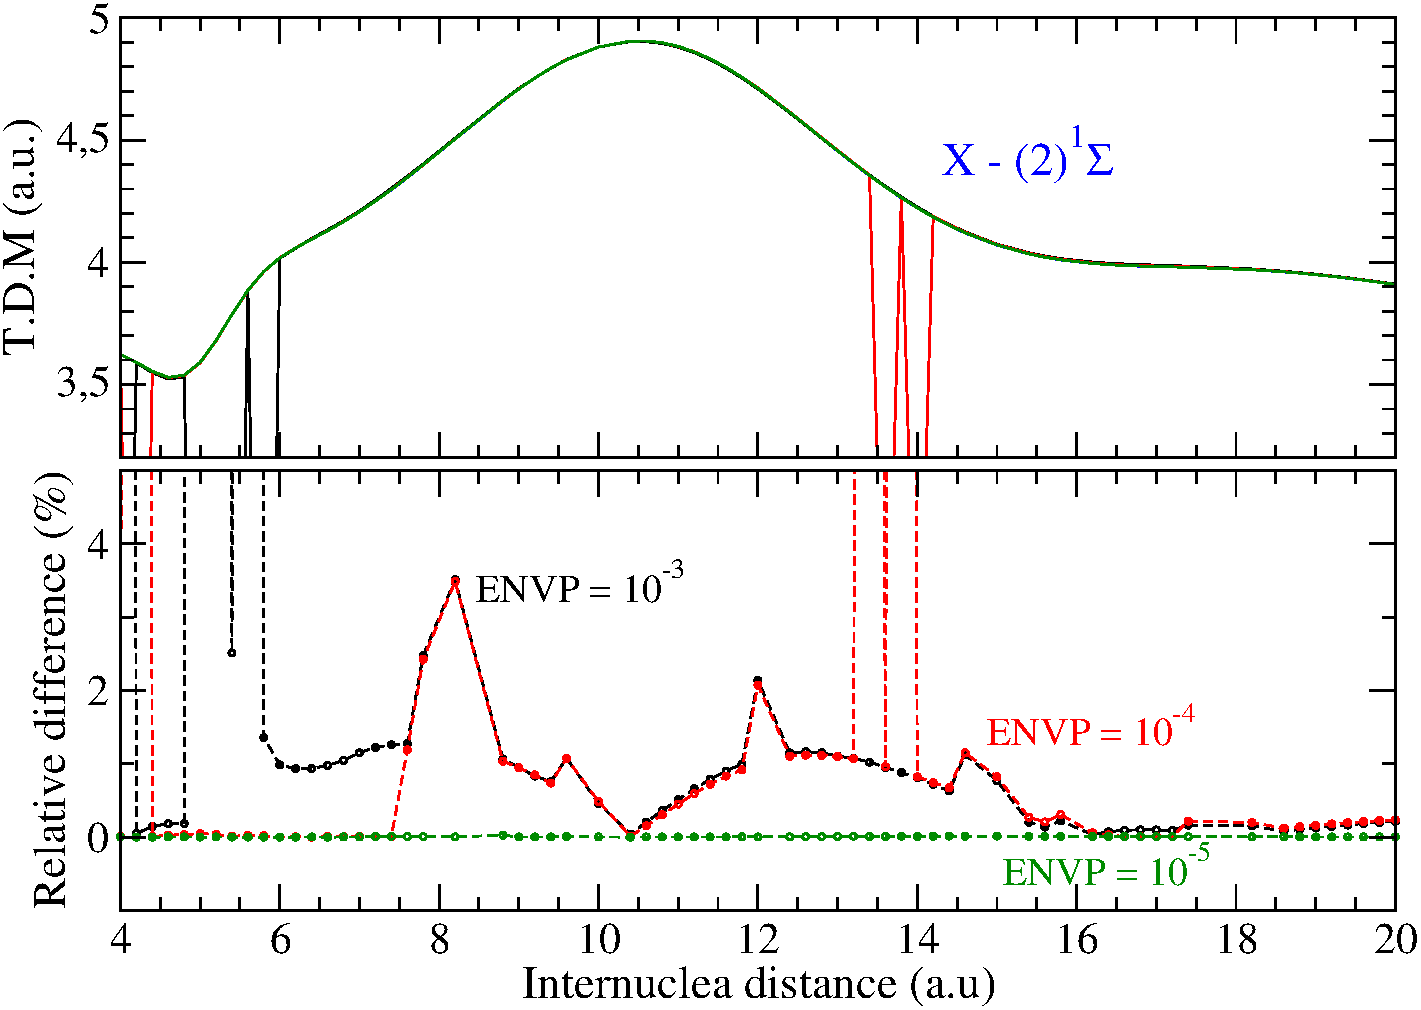
\includegraphics[width=0.8\textwidth]{fig/tdm_2ssp.pdf}
    \caption{\label{tdm2} \small Same as fig. \ref{tdm1} but for X-A tdm.}
  \end{center}
\end{figure*}

\pagebreak


\begin{table*}[htbp]
  \begin{center}
 \begin{tabular}{|c|c|c|c|c|}
 \hline
State &\multicolumn{2}{|c|}{FCI PECs} & \multicolumn{2}{|c|}{CIPSI PECs} \\
& Diss. Energy &  $C_6$ & Diss. Energy &  $C_6$ \\
 \hline
$(1)^1\Sigma^+$ & -0.302620 & 7601.61 & -0.302620 & 7601.82 \\
$(2)^1\Sigma^+$ & -0.249999 & 81862 & -0.249999 & 81864.5 \\
$(3)^1\Sigma^+$ & -0.243258 & -11938.3 & -0.243258 & -11930.4 \\
$(4)^1\Sigma^+$ & -0.236268 & 28589.6 & -0.236268 & 28579.1 \\
$(1)^3\Sigma^+$ & -0.302620 & 7554.95 & 0.302620 & 7555.26 \\
$(2)^3\Sigma^+$ & -0.250001 & 77013.1 & -0.250001 & 77013.9 \\
$(3)^3\Sigma^+$ & -0.243262 & -14818.4 & -0.243262 & -14806.7 \\
$(4)^3\Sigma^+$ & -0.236283 & 19307.3 & -0.236283 & 19302.2 \\
$(8)^1\Sigma^+$ & -0.204280 & 261577 & -0.204278 & 262776 \\
 \hline
 \end{tabular}
 \caption{\label{londonv154} \small Fit of the longrange part of the PECs (from 25 to 30 a.u.) with the form $E_d - C_6/R^6$. } 
 \end{center}
\end{table*}

\pagebreak

\subsection{RbCa}

Using GMPCS, a test at $R=8~a.u.$ for $\Sigma$ symmetry gave the results in $2213~s$ using 57680 determinants for $ENVP=2.10^{-5}~a.u.$ and $25067~s$ using 214887 determinants for FCI.

On my laptop, a full calculation ($\Sigma$/$\Pi$/$\Delta$ + tdm) for a single point took $3790.8~s$. 

On GMPCS, ($\Sigma$/$\Pi$/$\Delta$) took $65441~s$ for a FCI.

 \begin{figure*}[ht!]
  \begin{center}
        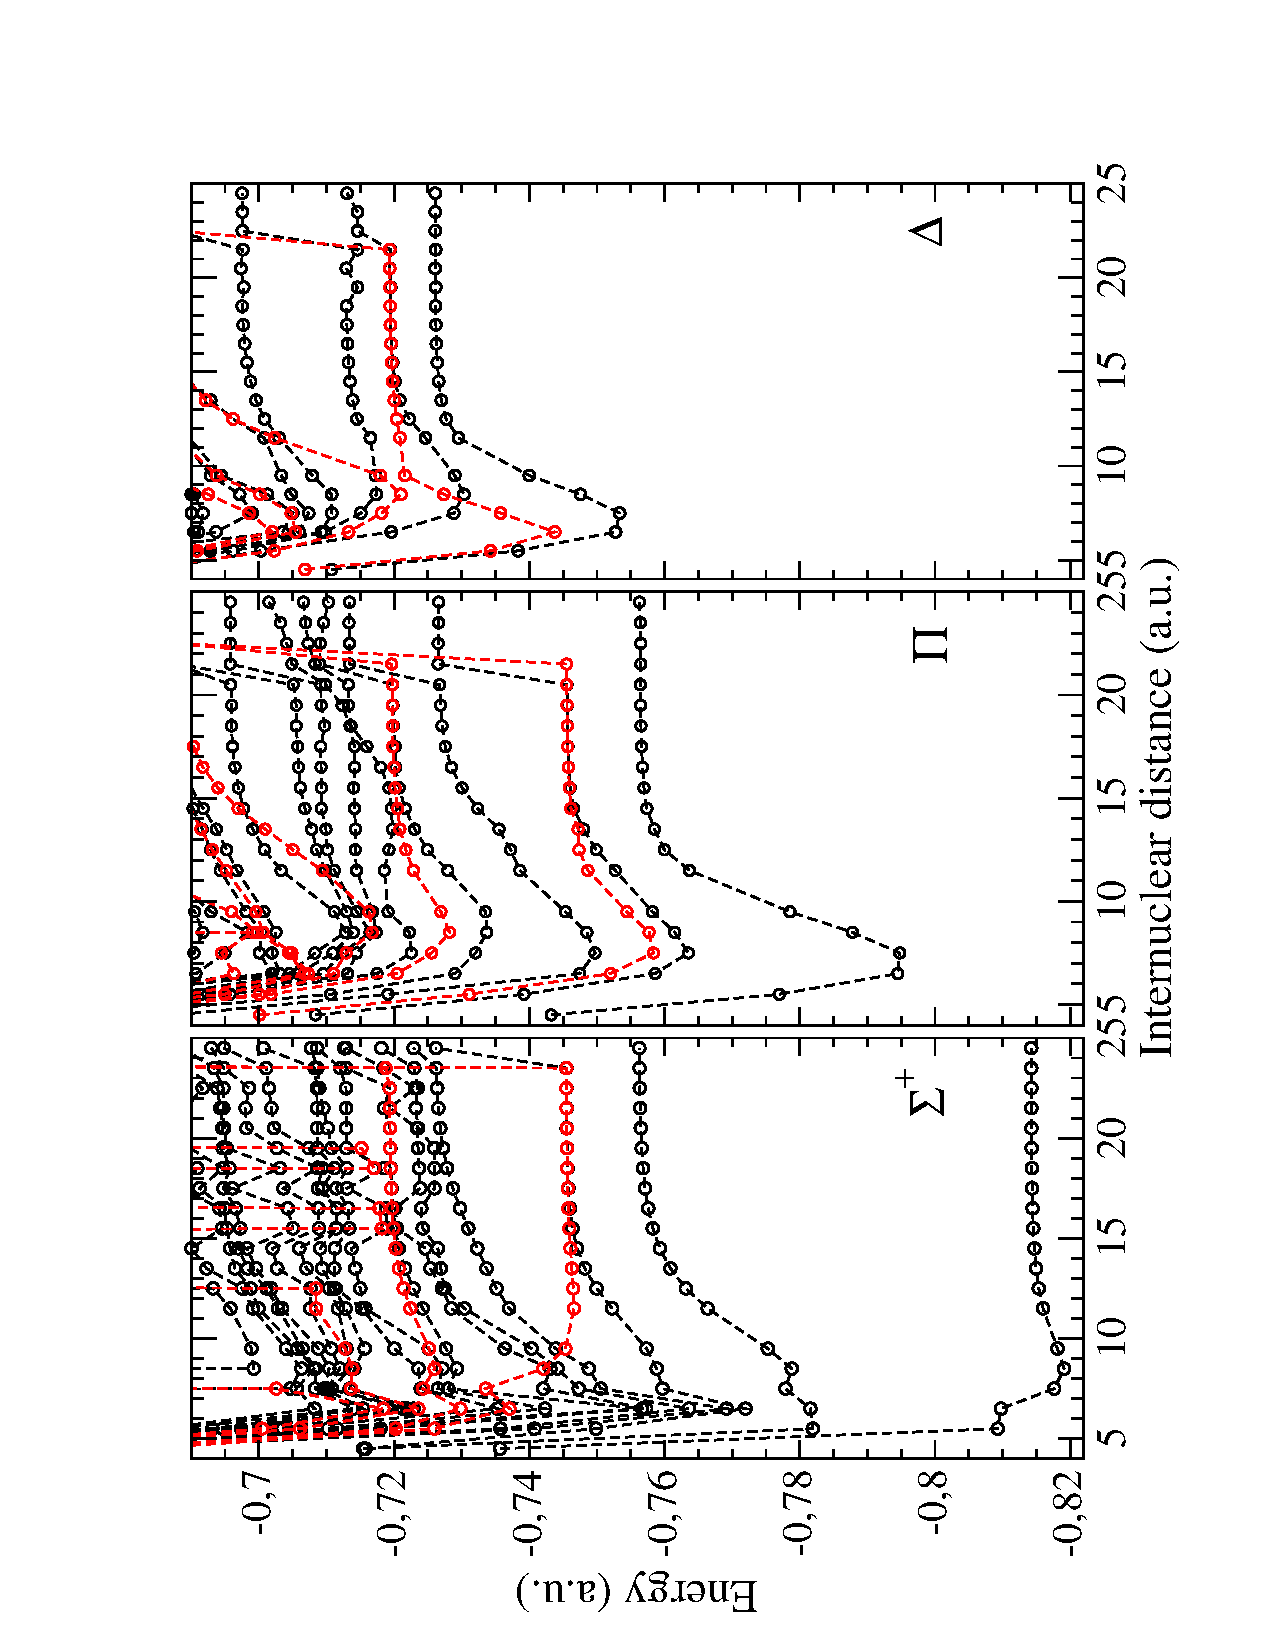
\includegraphics[angle=270,width=0.7\textwidth]{fig/RbCa_PECs.pdf}
    \caption{\label{pec_rbca} \small PEC computed for $ENVP=10^{-5}~a.u.$.}
  \end{center}
\end{figure*}


 \begin{figure*}[hb!]
  \begin{center}
        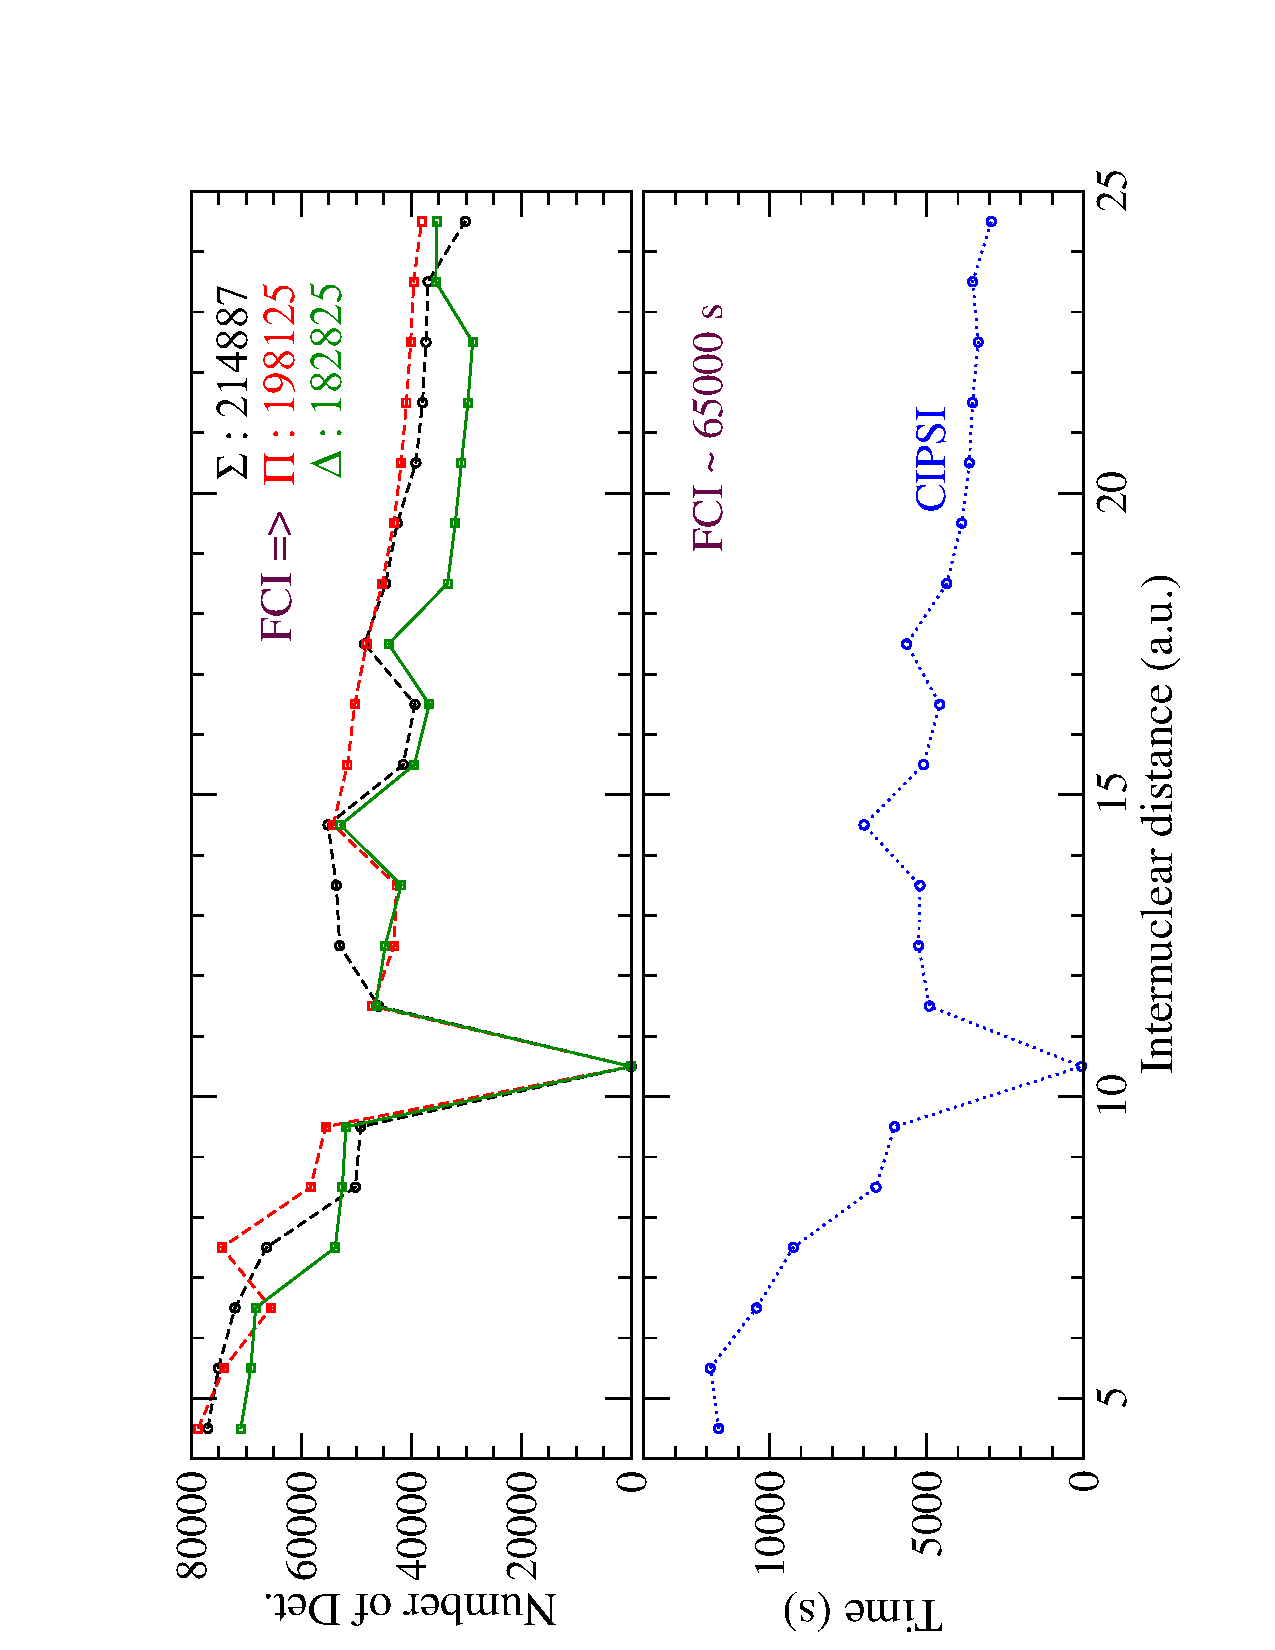
\includegraphics[angle=270,width=0.8\textwidth]{fig/time_GMPCS_RbCa.pdf}
    \caption{\label{time_l_rbca} \small Full calculation on GMPCS for 20 $\Sigma$/$\Pi$/$\Delta$. Number of determinants and computation time for each geometry ($ENVP=10^{-5}~a.u.$)}
  \end{center}
\end{figure*}

\end{document}
